%pdflatex -synctex=1 -interaction=nonstopmode gemaDOc.tex

\documentclass[a4paper, 11pt]{article}
\usepackage{setspace}
\setstretch{1.5}
\usepackage[ngerman]{babel}
\usepackage[utf8]{inputenc}
\usepackage{graphicx}

%Eurozeichen: €
\usepackage{eurosym} 
%raender kleiner machen
\usepackage{geometry}
\geometry{verbose,a4paper,bottom=3cm}

%Fußnoten ohne Nummern
\usepackage{nccfoots}
%Klickbare Links
%\usepackage[hidelinks]{hyperref}
\usepackage[hyphens]{url}
\usepackage{hyperref}
\usepackage{xcolor}
\hypersetup{
    colorlinks,
    linkcolor={blue!40!black},
    citecolor={blue!50!black},
    urlcolor={blue!60!black}
}

%umlgraphics
%\ifx\pdftexversion\undefined
%\usepackage[dvips]{graphicx}
%\else
%\usepackage[pdftex]{graphicx}
\DeclareGraphicsRule{*}{mps}{*}{}
%\fi

\usepackage{helvet}
\renewcommand{\familydefault}{\sfdefault}

\pagestyle{myheadings}
\markright{HAW Hamburg, Media Systems, SoSe 15}
\begin{document}
\newpage


\begin{verbatim}




\end{verbatim}
\begin{center}


\newcommand{\HRule}{\rule{\linewidth}{0.5mm}}
\HRule \\[0.4cm]
{ \huge \bfseries Entwicklerhandbuch}
\HRule

\Large{Natural Beverages Webshop} \\[1cm]

\begin{minipage}{0.55\textwidth}
\begin{flushleft} \large
\emph{Author:} \\
\emph{Matrikelnummer:} \\
\emph{Fach:} \\
\emph{Dozent:}
\end{flushleft}
\end{minipage}
\hfill
\begin{minipage}{0.4\textwidth}
\begin{flushright} \large
\emph{Author \textsc{A}} \\
\emph{42} \\
\emph{RDB} \\
\emph{Dozent \textsc{A}}
\end{flushright}
\end{minipage}
\end{center}
\begin{verbatim}



\end{verbatim}

\begin{abstract}
\noindent %kein eingerueckter Satz
Ein Entwicklertagebuch zum RDB Projekt \\ [1cm]
\end{abstract}

\newpage

\tableofcontents
\listoffigures

\newpage
%fragestellung, Einleitung, Relevanz
\section{Einleitung - Konzept}
Natural Beverages ist ein Webshop der sich auf \grqq natürliche\grqq  Getränke spezialisiert. Also Getränke aus Früchten, Getreide und anderen Rohstoffen. \\ 

Bio, FairTrade, lokale Ernährung sind aktuelle Stichworte und gerade zu Zeiten von Energy Drinks und Coca Cola hat sich eine Gruppe gefunden, die auf \grqq natürliche\grqq  Produkte besteht. In diesem Sinne stellt \grqq Natural Beverages\grqq  die Möglichkeit da auch lokale Sorten und Getränke zu kaufen. Hauptkategorien stellen Bier, Wein, Tees und Säfte.

Die Zielgruppe liegt als vor allem bei Jugendlichen, Mitte bis Ende 20, die sich sehr gut mit mobiler Technologie auskennen.
\section{Anleitung und Benutzung}
\begin{itemize}
\item \emph{Entweder} \grqq admin/databaseScript.sql\grqq \ in mysql mit dem Befehl \ \grqq source \grqq \ ausführen
\item \emph{oder} Servlets in \grqq public\_html/WEB-INF/classes/\grqq \ compilieren und mit \\ \grqq /localhost/admin/NBCreate.html\grqq \ ausführen.
\item Ab hier lässt sich die Website (localhost:8080/) benutzen.
\item Oben rechts auf den Menüschalter, auf \grqq Sign Up\grqq  und dann Daten eingeben.
\item links neben dem Menü lassen sich Email und Passwort zum Registrieren eingeben.
\item Nun können die Daten geändert oder unter Menü->Products Produkte zum Warenkorb hinzugefügt werden.
\item Der Warenkorb wird ebenfalls im Menü->Cart geöffnet und kann hier bestätigt/ zurückgesetzt/ angeschaut werden.
\item nach erfolgreicher Bestellung lässt sich diese unter Menü->Settings einsehen.
\item Mit dem Ausloggen mittels des Schalters links neben den Einstellungen (oder via Menü) ist das Programm komplett.
\end{itemize}
\section{Webseiten Design}

\subsection{Design}
Zum Darstellen der Elemente wird das CSS Framework Materialize (\url{http://materializecss.com/about.html}) genutzt. Begründung dafür liegt in der Zielgruppe. Es ist davon auszugehen, dass sich die Zielgruppe im Apple- oder im Googleumfeld bewegt. Android, iOS sind die Stichworte dieser Generation. Materalize holt das Webdesign in das aktuelle Aussehen von Google Software(Wie zum Beispiel auch das aktuelle Android 5). \\

Gleichzeitig braucht das Design eine Note rustikal. Natur als Thema mit Technologie. Also grüne, braune Akzente.
Ein dunkler Hintergrund hebt die hellen, freien Inhalte hervor. 

\subsection{Wege}
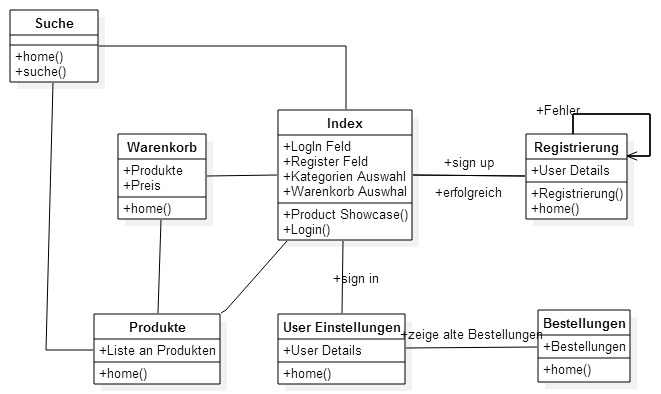
\includegraphics[width=\textwidth]{websiteWege.jpg}
\section{Programmtechnisches Design}

\subsection{Datenbank}
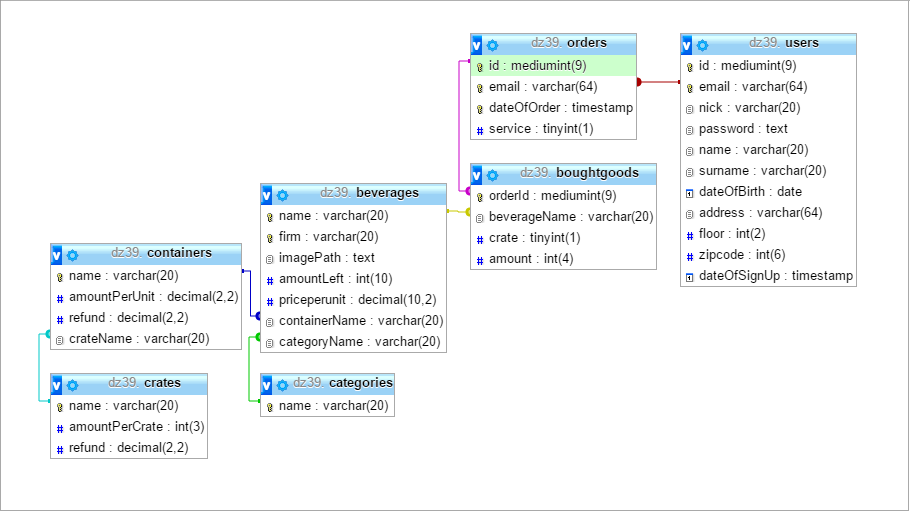
\includegraphics[width=\textwidth]{databaseDiagram.PNG}
Bei der Datenbank wurde auf den Verzicht von Id's geachtet. Id's machten letztendlich nur bei den Orders, sowie den Users Sinn da, ein User am Tag mehrmals das gleiche bestellen kann und Date für einen Primary Key etwas unhandlich ist. Außerdem könnte sich die Email eines Users ändern. \\
Im Grunde teilt sich die Datenbank in drei Teile auf. Orders und Boughtgoods vereinigen dabei alle anderen: eine Bestellung eines Users enthällt gekaufte Produkte mit Anzahl und Preis welche wiederum auf das Produkt zugreifen. Produkt, Category, Crate und Container beschreiben damit das Produkt insgesamt mit allen Anteilen. \\
Es lässt sich darüber streiten ob ein solche Datenbankkonstrukt in der reellen Welt einsatzbereit ist. Sobald eine Kategorie umbenannt werden soll entsteht ein riesiger Schaden, da das nicht einfach so geschehen kann, ohne das Informationen verloren gehen können. Mit einer id als Primary Key wäre dies jedoch ohne weiteres möglich.
\subsection{Dateistruktur}
\begin{itemize}
\item doc - enthällt die Dokumentation (also Hauptsächlich dieses File, Graphen, ...).
\item webapps/jsp - das eigentliche Programm, welches so auch im Praxi zu finden ist.
	\begin{itemize}
		\item admin - die Adminverwaltungsservlets zur Stammdatenverwaltung (siehe Admin Tool).
		\item css - die Stylesheets für die Website
		\item font - weitere Fonts für die Website (gehören zu materialize).
		\item images - Die Bilder der Website images/products für die Produkte.
		\item modules - enthällt die jsp Seiten(teile)
		\item scripts - Javascriptscripte zum Darstellen von dynamischen Inhalten.
		\item WEB-INF/classes - enthällt sowohl die servlet Klassen, als auch die Datenbankfiles.
	          Außerdem wurden hier nochmal die *.jars aus /WEB-INF/lib/ reinentpackt.
		\item WEB-INF/lib - enthällt eine json Lib (Die sollte bei einer aktuellen(!) Javaversion bereits vorhanden sein)
	\end{itemize}
\end{itemize}


\subsection{Authentication und User Management}
Ein LogIn geschieht über einen Abruf und Abgleich der Datenbank. Das eingegebene Passwort wird in md5 gehasht und anschließen mit dem Datenbankeintrag (ebenfalls md5) abgeglichen.
Vermutlich würde man in der reellen Welt eine bessere Hashingmethode verwenden. Beim erfolgreichen Einloggen wird der Session eine Variable("id") gesetzt. \\
Ausloggen ist einfach nur das Entfernen dieser Variable.\\
Die Ursprüngliche Idee war einen Filter(siehe /WEB-INF/NaturalBeverages/SessionFilter.java) zu benutzen. Sofern die SessionVariable \grqq nick\grqq \ (die beim einloggen gesetzt wurde) nicht null beträgt, wird der Client auf die angeforderte Seite weiter- oder ansonsten auf eine Fehlerseite geführt. Problem daran ist, dass auf dem Produktionsserver (praxi) Annotations nicht funktionieren und die web.xml auch nicht anfassbar war, da diese nur bei einem Serverneustart neu eingelesen wurde. \\
Somit dient eine einfache Abfrage über jeder entsprechenden Seite zur Kontrolle der Authentikation.  

\subsection{Admin Tool}
Das \grqq Admin Tool\grqq  ist ein auf Servlets basierendes Webtool mit dem sich Produkt Einträge aus der Datenbank hinzufügen und löschen lassen. Die Admintools werden durch den Zugriff auf /admin erreicht. 

\section{Reflektion und Fazit}
Die Seite hat noch einige Baustellen. Zu den Produkten ließe sich eine allgemeine Übersicht, eine Suche hinzufügen. Die Adminverwaltung hätte besser ausfallen können (Listen auswählen, statt Text suchen). Es fehlt an gutem Design.\\

Außerdem ist das System der Anbindung nicht ganz durchdacht: Product.java dient nur als Halter für ein Produkt, zum Speichern des Warenkorbs wird dieses nochmal neu erstellt. Sinvoller wäre es gewesen mit einer jsp Seite eine Klasse Products.java auszugeben, die die Produkte abgespeichert hat. \\

Die Arbeit mit den Servlets ist recht umständlich und selbst JSP Seiten kommen nicht an die Bequemlichkeit von Sinatra/Ruby On Rails Applications heran. \\
Da durchgängig Probleme mit dem VPN, sowie Praxi(jsp Seiten wurden ständig gecached), gestaltete sich die Arbeit teilweise als Problematisch. Auf dem eigenem Netzwerk war die 
Arbeit aber durchaus sehr interessant. 
\section{User Stories}
\begin{itemize}
	\item As a client I want to browse the baverages of the shop
	\item As an older person I want the delivery service to carry my items into my apartment
	\item As a client I want to get a bill at the end of the order with the given address
		- I also want to see:
			- glass and crate refunds
			- delivery-into-apartment price per litre
	\item As a client I want to be able to find the beverages I am looking for
	\item As a client I want to be able to view a help page
	\item I want to have the comfort of a user account to store previous orders
	\end{itemize}
\end{document}
